El sistema no lleva un proceso de instalaci\'on arduo, simplemente es necesario copiarlo en una computadora que cumpla con los requisitos previamente expuestos. Para usarse s\'olo se requiere abrir el archivo que se muestra a continuaci\'on.
\begin{figure}[htbp!]
\centering
		
\includegraphics[width=.8\textwidth]{images/archivo}
		\caption{Archivo a ejecutar (Ejecutable JAR)}
	\end{figure}
	
Una buena sugerencia es que se cree un acceso directo al escritorio del ejecutable, dando click derecho al mismo y escogiendo la opci\'on mostrada en la siguiente figura.

\begin{figure}[htbp!]
\centering
		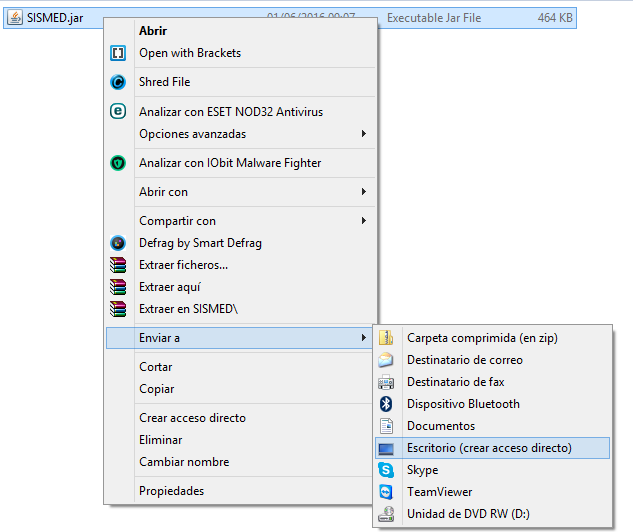
\includegraphics[width=.8\textwidth]{images/acceso}
		\caption{Creaci\'on de acceso directo al escritorio}
	\end{figure}
